\chapter{Исследовательская часть}

В этой части представлены технические характеристики ЭВМ, а также
результаты исследования зависимости времени построения изображения
ландшафта от размера карты высот.


\section{Технические характеристики ЭВМ}

Все замеры проводились на ЭВМ, характеристики которой приведены
ниже:

\begin{itemize}
    \item процессор: AMD Ryzen™ 7--5800H with Radeon™ Graphics × 16, 3.8 ГГц~\cite{radeon};
    \item ОС: 64-разрядная операционная система Ubuntu 24.04.1 LTS~\cite{ubuntu};
    \item оперативная память: 16,0 ГБ;
    \item число логических ядер -- 16.
\end{itemize}

\section{Результаты исследования}

В ходе эксперимента производилось построение квадратных карт высот
различных размеров, построение полигональной модели по построенной карте.
Далее измерялось время рендеринга полученной полигональной сетки.
Время замерялось с помощью функции $std::chrono::high\_resolution\_clock::now$~\cite{clock} из стандартной библиотеки $<chrono>$~\cite{chrono}.
Для каждой размерности было произведено 100 замеров. Время
отрисовки ландшафта не учитывалось. Полученные результаты, после нахождения среднего значения,
представлены в таблице~\ref{table:rendering_times}.

\begin{table}[H]
    \centering
    \caption{Среднее время рендеринга сцены в зависимости от размера высотной карты.}
    \begin{tabular}{|c|r|}
        \hline
        \textbf{Размерность карты высот} & \textbf{Среднее время рендеринга (мс)} \\ \hline
        30 & 1.13 \\ \hline
        60                               & 19.77                                  \\ \hline
        90                               & 45.22                                  \\ \hline
        120                              & 97.95                                  \\ \hline
        150                              & 123.46                                 \\ \hline
        180                              & 155.18                                 \\ \hline
        210                              & 183.96                                 \\ \hline
        240                              & 218.67                                 \\ \hline
        270                              & 254.64                                 \\ \hline
        300                              & 298.73                                 \\ \hline
    \end{tabular}
    \label{table:rendering_times}
\end{table}

На рисунке~\ref{img:plot} представлена визуализация результатов.
График построен при помощи библиотеки $Python$ $matplotlib$~\cite{plot}.

\begin{figure}[H]
	\centering
	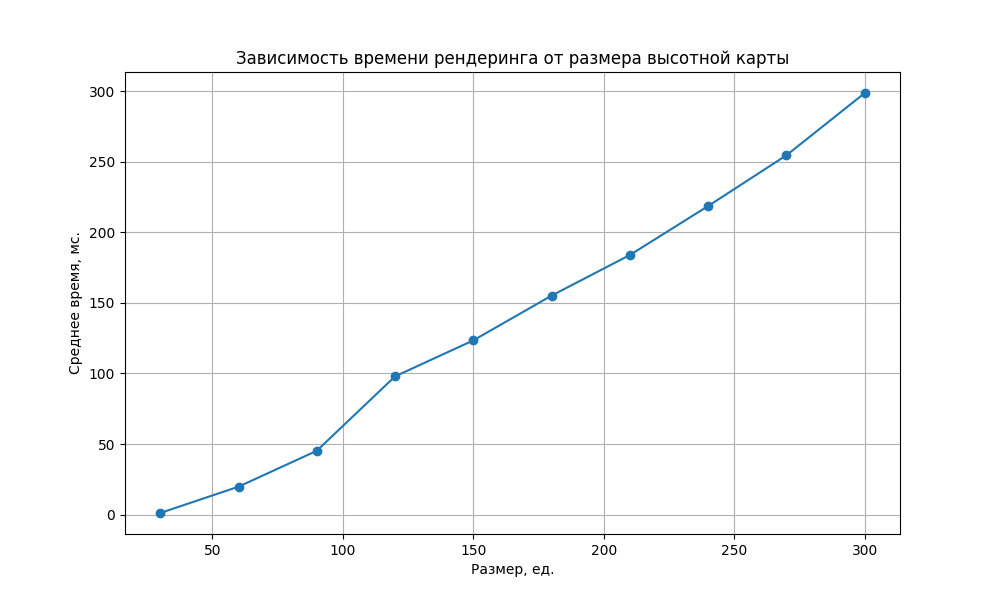
\includegraphics[scale=0.5]{images/render}
	\caption{Зависимость времени рендеринга от размера высотной карты}
	\label{img:plot}
\end{figure}

Из графика можно сделать вывод, что зависимость времени построения изображения ландшафта от размера квадратной
карты высот линейна.

\section*{Вывод}

В данном разделе описаны технические характеристики ЭВМ, на которой проводился эксперимент,
а также представлены ход выполнения эксперимента и его результаты. Полученные данные подтвердили ожидания:
время построения изображения ландшафта линейно зависит от размера квадратной карты высот, что соответствует
теоретической сложности алгоритма с использованием Z-буфера.